\begin{table}[H]
\centering
\begin{tabular}{|l|l|l|l|l|}
\hline 
\textbf{Clasificación} & \textbf{Total} & \textbf{Aciertos} & \textbf{Errores} & \textbf{Eficiencia} \\
\hline
Estado & 1393 & 670 & 723 & 48.097 \\
\hline 
Categoría & 1393 & 259 & 1134 & 18.592 \\
\hline 
\end{tabular}
\caption{Eficiencias generales con Hue 40-80}
\label{table:efficiency_general_40_80}
\end{table}

\captionsetup[figure]{skip=-10pt}

\begin{figure}[H]
\centering
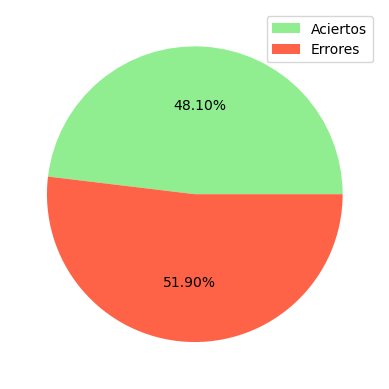
\includegraphics[scale=0.6]{images/result_global_state_40_80.png}
\caption{Eficiencia detectando el estado con Hue 40-80}
\label{img:efficiency_state_40_80}
\end{figure}

\begin{figure}[H]
\centering
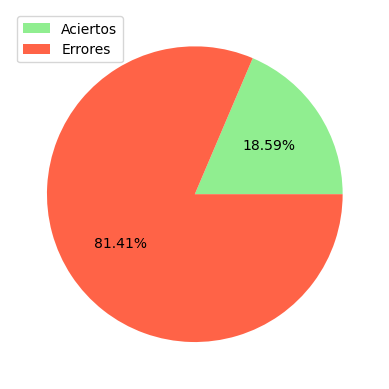
\includegraphics[scale=0.6]{images/result_global_class_40_80.png}
\caption{Eficiencia detectando la categoría con Hue 40-80}
\label{img:efficiency_category_40_80}
\end{figure}

\captionsetup[figure]{skip=10pt}

\begin{table}[H]
\centering
\begin{tabular}{|l|c|c|c|}
\hline 
\textbf{Categoría} & \textbf{Original} & \textbf{Calculado} & \textbf{Eficiencia} \\
\hline
healthy & 791 & 75 & 9.481 \\
\hline 
rust\_level\_1 & 344 & 77 & 22.383 \\
\hline 
rust\_level\_2 & 166 & 73 & 43.975 \\
\hline 
rust\_level\_3 & 62 & 22 & 35.483 \\
\hline 
rust\_level\_4 & 30 & 12 & 40.0 \\
\hline 
\end{tabular}
\caption{Eficiencia por categoría con Hue 40-80}
\label{table:efficiency_categories_40_80}
\end{table}

\begin{figure}[H]
\centering
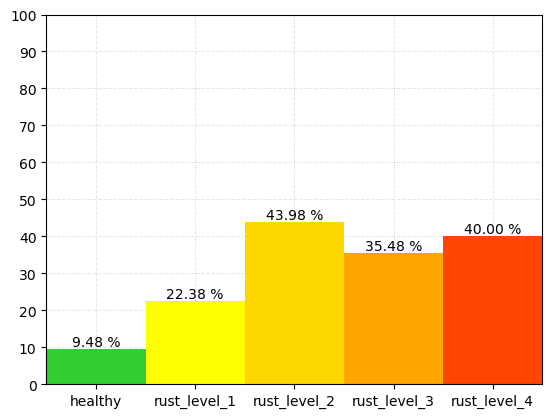
\includegraphics[scale=0.6]{images/result_classes_40_80.png}
\caption{Eficiencia por categoría con Hue 40-80}
\label{img:efficiency_categories_40_80}
\end{figure}
